%% AMS-LaTeX Created by Wolfram Mathematica 7.0 : www.wolfram.com

\documentclass{article}
\usepackage{amsmath, amssymb, graphics}

\newcommand{\mathsym}[1]{{}}
\newcommand{\unicode}{{}}

\begin{document}

\noindent\(\pmb{\text{Options}[\text{Singularity}]=\{\text{Angle}\to \text{Pi}/3,\text{Even}\to \text{True}\};}\\
\pmb{\text{Singularity}[\text{pt1$\_$List},\text{pt2$\_$List},\text{width$\_$},\text{options$\_\_\_$}]\text{:=}\text{Line}[\text{Module}[\{\text{vecL},\text{vecT},n,}\\
\pmb{\text{length}=\text{Sqrt}[(\text{pt2}-\text{pt1}).(\text{pt2}-\text{pt1})],}\\
\pmb{\text{relangle}=\text{Angle}\text{/.}\text{Flatten}[\{\text{options}\},1]\text{/.}\text{Options}[\text{Singularity}],}\\
\pmb{\text{even}=\text{Even}\text{/.}\text{Flatten}[\{\text{options}\},1]\text{/.}\text{Options}[\text{Singularity}]\},}\\
\pmb{n=\text{Round}[\text{length}/(2\text{width} \text{Tan}[\text{relangle}/2])]+\text{If}[\text{even},0,1];}\\
\pmb{\text{vecL}=(\text{pt2}-\text{pt1})/n;}\\
\pmb{\text{vecT}=\{-\text{$\#$1},\text{$\#$2}\}\&\text{@@}\text{Reverse}[\text{vecL}];}\\
\pmb{\text{vecT}=\text{vecT}/\text{Sqrt}[\text{vecT}.\text{vecT}]\text{width};}\\
\pmb{\{\text{pt1}\}\sim \text{Join}\sim \{\text{pt1}+\text{vecL}\}\sim \text{Join}\sim \text{Table}[\text{pt1}+(i+1/2) \text{vecL}-(-1){}^{\wedge}i
\text{vecT},\{i,1,n-2\}]\sim }\\
\pmb{\text{Join}\sim \{\text{pt2}-\text{vecL}\}\sim \text{Join}\sim \{\text{pt2}\}}\\
\pmb{]]}\)

\noindent\(\pmb{\text{Show}[\text{Graphics}[\{}\\
\pmb{\{\text{Thickness}[.002],\text{Line}[\{\{0,0\},\{0,3\}\}]\},}\\
\pmb{\{\text{Thickness}[.002],\text{Line}[\{\{0,0\},\{0,-3\}\}]\},}\\
\pmb{\{\text{Thickness}[.002],\text{Line}[\{\{3,0\},\{0,0\}\}]\},}\\
\pmb{\{\text{Thickness}[.002],\text{Line}[\{\{-3,0\},\{0,0\}\}]\},}\\
\pmb{\{\text{PointSize}[.025],\text{Black},\text{Point}[\{2,2\}]\},}\\
\pmb{\{\text{PointSize}[.025],\text{Black},\text{Point}[\{2,-2\}]\},}\\
\pmb{\{\text{PointSize}[.025],\text{Black},\text{Point}[\{2,0\}]\},}\\
\pmb{\{\text{Thickness}[.002],\text{Circle}[\{2,2\},.5,\{-2.50,2.50\}]\},}\\
\pmb{\{\text{Thickness}[.002],\text{Circle}[\{2,-2\},.5,\{-2.50,2.50\}]\},}\\
\pmb{\{\text{Thickness}[.002],\text{Line}[\{\{1.60,2.30\},\{-2,2.30\}\}]\},}\\
\pmb{\{\text{Thickness}[.002],\text{Line}[\{\{1.60,1.70\},\{-2,1.70\}\}]\},}\\
\pmb{\{\text{Thickness}[.002],\text{Line}[\{\{1.60,-2.30\},\{-2,-2.30\}\}]\},}\\
\pmb{\{\text{Thickness}[.002],\text{Line}[\{\{1.60,-1.70\},\{-2,-1.70\}\}]\},}\\
\pmb{\{\text{Thickness}[.002],\text{Black},\text{Singularity}[\{2,2\},\{-2,2\},.05]\},}\\
\pmb{\{\text{Thickness}[.002],\text{Black},\text{Singularity}[\{-2,-2\},\{2,-2\},.05]\},}\\
\pmb{\{\text{Arrowheads}[.025],\text{Arrow}[\{\{0,2.95\},\{0,3\}\}]\},}\\
\pmb{\{\text{Arrowheads}[.025],\text{Arrow}[\{\{2.95,0\},\{3,0\}\}]\},}\\
\pmb{\{\text{Arrowheads}[.025],\text{Arrow}[\{\{2,2.5\},\{2.25,2.45\}\}]\},}\\
\pmb{\{\text{Arrowheads}[.025],\text{Arrow}[\{\{2,-2.50\},\{1.95,-2.51\}\}]\},}\\
\pmb{\{\text{Arrowheads}[.025],\text{Arrow}[\{\{-1,2.2980\},\{-0.75,2.2980\}\}]\},}\\
\pmb{\{\text{Arrowheads}[.025],\text{Arrow}[\{\{-1,-2.2980+0.60\},\{-0.75,-2.2980+0.60\}\}]\},}\\
\pmb{\{\text{Arrowheads}[.025],\text{Arrow}[\{\{-0.90,-2.2980\},\{-0.95,-2.2980\}\}]\},}\\
\pmb{\{\text{Arrowheads}[.025],\text{Arrow}[\{\{-0.90,2.2980-0.6\},\{-0.95,2.2980-0.6\}\}]\},}\\
\pmb{\text{Text}\left[\texttt{"}n^2\texttt{"},\{2,0.25\}\right],\text{Text}[\text{$\texttt{"}$Im(z)$\texttt{"}$},\{0.33,2.85\}],\text{Text}[\text{$\texttt{"}$Re(z)$\texttt{"}$},\{2.75,0.2\}],}\\
\pmb{\text{Text}\left[\texttt{"}\delta _1\left(\tau _1,\tau _2\text{)$\texttt{"}$}\right.,\{2,1.33\}\right],\text{Text}\left[\texttt{"}\delta _2\left(\tau
_1,\tau _2\text{)$\texttt{"}$}\right.,\{2,-1.33\}\right],\text{Text}\left[\texttt{"}\epsilon _1^+\left(\tau _1,\tau _2\text{)$\texttt{"}$}\right.,\{-2,2.50\}\right],}\\
\pmb{\text{Text}\left[\texttt{"}\epsilon _1^-\left(\tau _1,\tau _2\text{)$\texttt{"}$}\right.,\{-2,1.50\}\right],\text{Text}\left[\texttt{"}\epsilon
_2^-\left(\tau _1,\tau _2\text{)$\texttt{"}$}\right.,\{-2,-2.50\}\right],}\\
\pmb{\text{Text}\left[\texttt{"}\epsilon _2^+\left(\tau _1,\tau _2\text{)$\texttt{"}$}\right.,\{-2,-1.50\}\right],}\\
\pmb{\{\text{Thickness}[.001],\text{Circle}[\{2,0\},.5,\{-2.50,2.50\}]\},}\\
\pmb{\{\text{Thickness}[.001],\text{Line}[\{\{1.60,0.30\},\{-1.6,.30\}\}]\},}\\
\pmb{\{\text{Thickness}[.001],\text{Line}[\{\{1.60,-0.30\},\{-1.6,-.30\}\}]\}}\\
\pmb{\text{                                                 }\}],}\\
\pmb{\text{PlotRange}\to \{\{-3.00,3.00\},\{-3.00,3.00\}\},\text{AspectRatio}\to \text{Automatic}]}\)

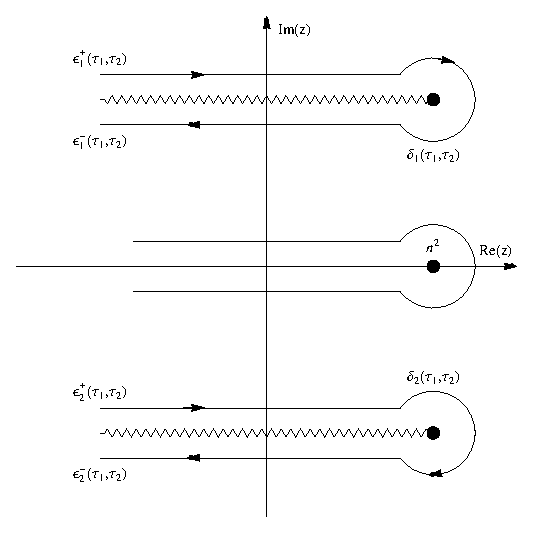
\includegraphics{ContoursPlots_gr1.eps}

\noindent\(\pmb{\text{Show}[\text{Graphics}[\{}\\
\pmb{\{\text{Thickness}[.002],\text{Line}[\{\{-2,0\},\{-2,3\}\}]\},}\\
\pmb{\{\text{Thickness}[.002],\text{Line}[\{\{-2,0\},\{-2,-3\}\}]\},}\\
\pmb{\{\text{Thickness}[.002],\text{Line}[\{\{-3,0\},\{3,0\}\}]\},}\\
\pmb{\{\text{Thickness}[.004],\text{Line}[\{\{2,0\},\{2,3\}\}]\},}\\
\pmb{\{\text{Thickness}[.004],\text{Line}[\{\{2,0\},\{2,-3\}\}]\},}\\
\pmb{\{\text{Thickness}[.004],\text{Line}[\{\{2,0\},\{2,-3\}\}]\},}\\
\pmb{\{\text{Thickness}[.002],\text{Black},\text{Singularity}[\{0,0\},\{0,3\},.05]\},}\\
\pmb{\{\text{Thickness}[.002],\text{Black},\text{Singularity}[\{0,0\},\{0,-3\},.05]\},}\\
\pmb{\{\text{PointSize}[.007],\text{Black},\text{Point}[\{1,1\}]\},}\\
\pmb{\{\text{PointSize}[.007],\text{Black},\text{Point}[\{1,-1\}]\},}\\
\pmb{\text{Text}[\text{$\texttt{"}$Re(s)$\texttt{"}$},\{2.75,0.2\}],\{\text{Arrowheads}[.025],\text{Arrow}[\{\{-2,2.95\},\{-2,3\}\}]\},}\\
\pmb{\{\text{Arrowheads}[.025],\text{Arrow}[\{\{2.95,0\},\{3,0\}\}]\},\text{Text}[\text{$\texttt{"}$Im(s)$\texttt{"}$},\{-2.33,2.85\}],}\\
\pmb{\text{Text}\left[\text{$\texttt{"}$Re(s)=}\frac{1}{2}\texttt{"},\{-0.5,0.25\}\right],\text{Text}[\text{$\texttt{"}\rho $ = $\beta $ + i $\gamma
\texttt{"}$},\{1.2,0.75\}],\text{Text}\left[\texttt{"}\overline{\rho  }\text{= $\beta $ - i $\gamma \texttt{"}$},\{1.2,-0.75\}\right]}\\
\pmb{\text{                                                 }\}],}\\
\pmb{\text{PlotRange}\to \{\{-3.00,3.00\},\{-3.00,3.00\}\},\text{AspectRatio}\to \text{Automatic}]}\)

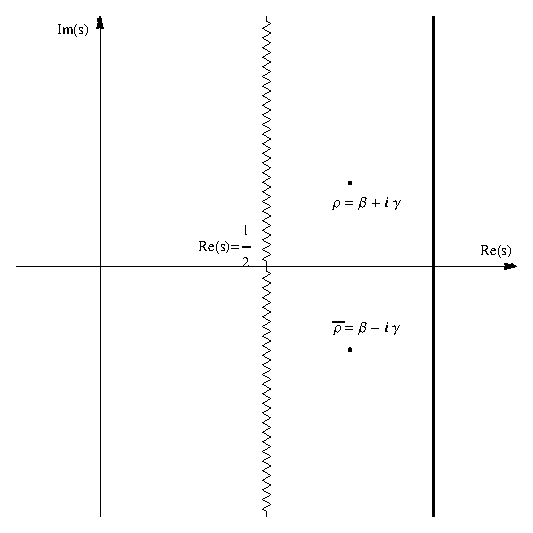
\includegraphics{ContoursPlots_gr2.eps}

\noindent\(\pmb{\text{Show}[\text{Graphics}[\{}\\
\pmb{\{\text{Thickness}[.002],\text{Line}[\{\{-3,0\},\{3,0\}\}]\},}\\
\pmb{\{\text{Thickness}[.002],\text{Line}[\{\{0,-3\},\{0,3\}\}]\},}\\
\pmb{\{\text{Thickness}[.004],\text{Line}[\{\{-1.5,-2.5\},\{-1.5,2.5\}\}]\},}\\
\pmb{\{\text{Thickness}[.004],\text{Line}[\{\{2.5,-2.5\},\{2.5,2.5\}\}]\} ,}\\
\pmb{\{\text{Thickness}[.004],\text{Line}[\{\{-1.5,-2.5\},\{2.5,-2.5\}\}]\} ,}\\
\pmb{\{\text{PointSize}[.007],\text{Black},\text{Point}[\{2,0\}]\},}\\
\pmb{\{\text{PointSize}[.007],\text{Black},\text{Point}[\{-2,0\}]\},}\\
\pmb{\{\text{Thickness}[.004],\text{Line}[\{\{-1.5,2.5\},\{2.5,2.5\}\}]\} ,\text{Text}[\text{$\texttt{"}$Im(s)$\texttt{"}$},\{0.33,2.85\}],}\\
\pmb{\text{Text}[\text{$\texttt{"}$Re(s)$\texttt{"}$},\{2.75,0.2\}],\text{Text}[\text{$\texttt{"}$1$\texttt{"}$},\{2.2,0.2\}],\text{Text}[\text{$\texttt{"}$-1$\texttt{"}$},\{-2,0.2\}],}\\
\pmb{\text{Text}[\text{$\texttt{"}$Re(s) = $\sigma \texttt{"}$},\{2,-1.2\}],\text{Text}[\texttt{"}\Omega \texttt{"},\{-1.75,2\}],\text{Text}[\text{$\texttt{"}$Re(s)
= $\eta \texttt{"}$},\{-2,-1.2\}],}\\
\pmb{\{\text{Arrowheads}[.025],\text{Arrow}[\{\{0,2.95\},\{0,3\}\}]\},}\\
\pmb{\{\text{Arrowheads}[.025],\text{Arrow}[\{\{2.95,0\},\{3,0\}\}]\},}\\
\pmb{\{\text{Arrowheads}[.025],\text{Arrow}[\{\{2.5,0\},\{2.5,1\}\}]\},}\\
\pmb{\{\text{Arrowheads}[.025],\text{Arrow}[\{\{1,2.5\},\{0.5,2.5\}\}]\},}\\
\pmb{\{\text{Arrowheads}[.025],\text{Arrow}[\{\{-1.5,0\},\{-1.5,-1\}\}]\},}\\
\pmb{\{\text{Arrowheads}[.025],\text{Arrow}[\{\{0.5,-2.5\},\{1,-2.5\}\}]\}}\\
\pmb{\}],}\\
\pmb{\text{PlotRange}\to \{\{-3.00,3.00\},\{-3.00,3.00\}\},\text{AspectRatio}\to \text{Automatic}]}\)

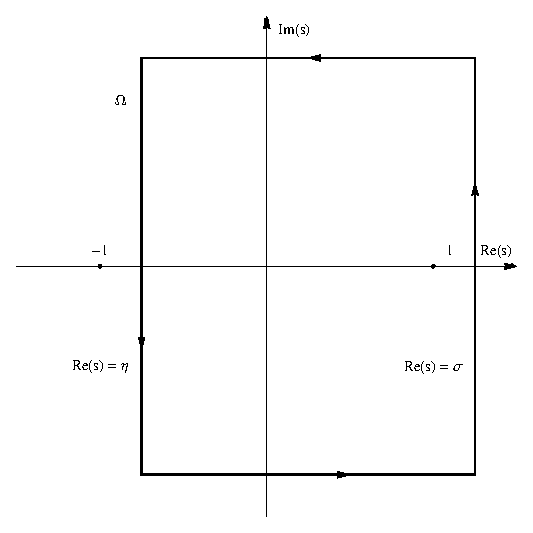
\includegraphics{ContoursPlots_gr3.eps}

\end{document}
